\section{이론적 배경}

\subsection{천체 관측 시스템}

Figure \ref{fig:observing_system}\은 관측 환경이 좋은 곳으로 망원경을 이동하여 사진 관측을 할 수 있는 소형 천체 망원경 시스템을 보여 준다. 사진 관측을 위한 천체 망원경 시스템은 크게 광학계(optic), 검출기(detector), 마운트(mount)로 이루어지며, 정밀도를 높이기 위해 가이드 시스템을 포함한 여러가지 보조 도구들이 필요하다. 광학계의 결상 성능, 마운트의 추적 성능 등을 갖추고 있어야 오랜 시간동안 노출을 주며 천체 사진을 찍을 수 있게 된다. 

앞서 제시한 Figure \ref{fig:The_Andromeda_Galaxy}의 안드로메다 은하 사진은 Figure \ref{fig:observing_system}\을 이용하여 촬영한 것이다. 상세 정보를 보면 Sbig(Santa Barbara Instrument Group)사의  ST-8300M이라는 모노크롬 CCD(Charge-coupled device)를 이용하여 촬영하였으며, 노출 정보를 보면 L(Luminence) 채널의 경우 600 sec의 노출로 14 frame을 촬영하여 합성하였으며, R(Red), G(Green), B(Blue) 각각의 채널에서 400 sec의 노출로 6 frame씩 촬영하여 합성한 것이다. 이처럼 고품질의 천체사진 한 장을 촬영하기 위해서 많은 시간과 노력이 필요하다. 

\begin{figure}[h]
	\begin{center}
		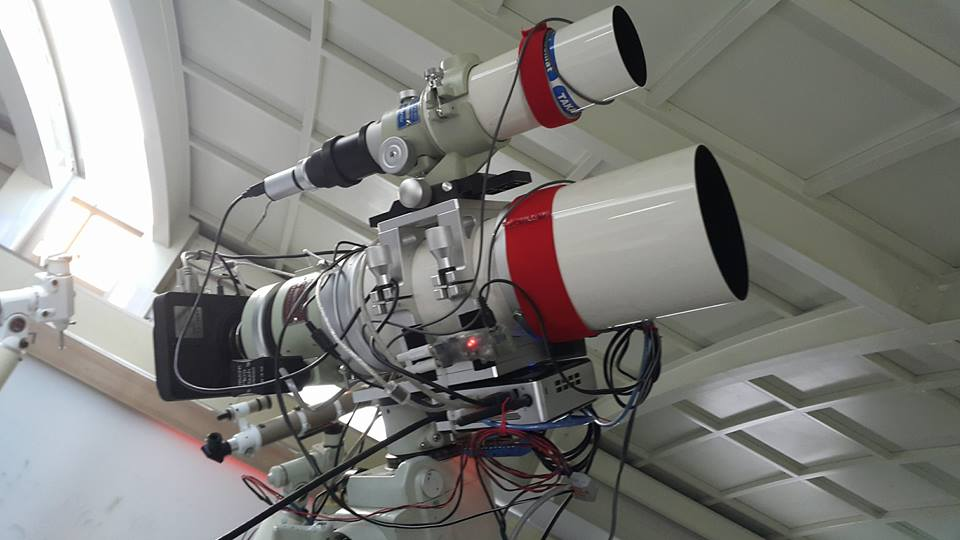
\includegraphics[width=0.8\linewidth]{observing_system}
		\caption{Telescope system for astrophotography}
		\label{fig:observing_system}
	\end{center}
\end{figure}

점 광원(Point light source)인 별빛은 대기

\subsection{자동 초점 조절}

이덕규 외(2014)는 복합재 광구조체와 결합하여 전자광학카메라의 영상 품질을 향상시킬 수 있는 초점 조절 장치를 개발하였다.\cite{leedukgu2014}\\
윤종환 외(2011)는 선명도에 관한 기울기를 이용하여 초점이 맞았는지를 확인하는 방법을 사용하였다.\cite{yunjonghwan2011lcd}\\
박석휘 외(2009)는 모바일 폰용 자동 초점 조절 알고리즘을 초점 값 계산 알고리즘을 이용하여 구현하였다.\cite{parksukhui2009Median}\\
이성희 외(1998)는 각 화소들의 미디언 값의 차이를 이용하여 초점을 맞추는 알고리즘을 구현하였다.\cite{leeseonghee1998Median}


\subsection{기존 제품 분석}

Figure \ref{fig:microtouch}\가 바로 미국의 Starizona사에서 판매하는 Micro Touch  제품이다. Figure \ref{fig:microtouch_3}\가 Micro Touch Autofocuser Hand Control system (Wired)이고, USB 케이블로 컴퓨터와 연결하여 ASCOM 호환 소프트웨어에서 제어가 가능하다.  Figure \ref{fig:microtouch_3}\는 Feather touch focuser에 모터를 장착한 모습이다. 장장ㅊ

%%%%%%%새로 그림 추가함 (박기현샘)

\begin{figure}[h]
	\begin{center}
		\begin{subfigure}{0.45\textwidth}
			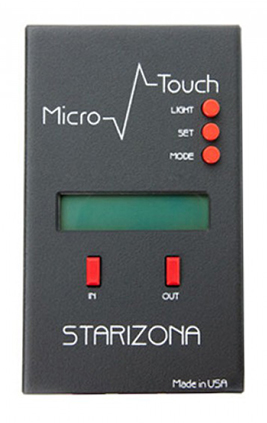
\includegraphics[width=0.9\linewidth]{microtouch_3} 
			\caption{Autofocuser Hand Control system (Wired)}
			\label{fig:microtouch_3}
		\end{subfigure}
		\begin{subfigure}{0.45\textwidth}
			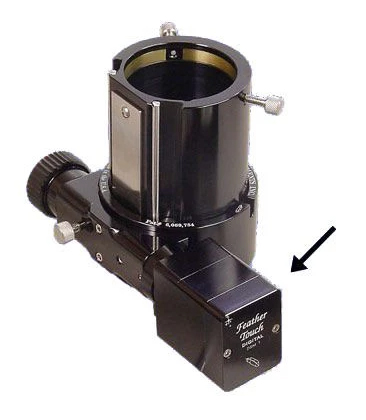
\includegraphics[width=0.9\linewidth]{microtouch_4}
			\caption{Feather touch focuser with motor}
			\label{fig:microtouch_4}
		\end{subfigure}
		\caption{Starizona사에서 판매하는 Micro touch 제품}
		\label{fig:microtouch}
	\end{center}
\end{figure}



수가 있다. Fig.2에서 나온 위의 두 버튼(IN, OUT)은 각각 초점을 맞추기 위해 망원경의 길이를 줄이거나 늘일 수 있는 버튼이다. Micro Touch를 수동 혹은 자동으로 작동시켜 IN 또는 OUT의 명령을 내렸을 경우, 모터 초점 조절 장치가 작동하게 된다. 이 모터 초점 조절 장치는 모터를 움직여 천체망원경의 경통의 길이를 조절할 수 있도록 한다. 경통의 길이가 변화하면 그에 따라서 빛이 퍼지는 정도가 달라지므로 이를 잘 조정하면 망원경으로 관측하는 천체의 초점을 맞출 수 있다.

\subsection{제품 설계}

\subsubsection{컨트롤러}

아두이노(이탈리아어: Arduino 아르두이노)는 오픈 소스를 기반으로 한 단일 보드 마이크로컨트롤러로 완성된 보드(상품)와 관련 개발 도구 및 환경을 말한다. 2005년 이탈리아의 IDII(Interaction Design Institutelvera)에서 하드웨어에 익숙지 않은 학생들이 자신들의 디자인 작품을 손쉽게 제어할 수 있게 하려고 고안된 아두이노는 처음에 AVR을 기반으로 만들어졌으며, 아트멜 AVR 계열의 보드가 현재 가장 많이 판매되고 있다. ARM 계열의 Cortex-M0(Arduino M0 Pro)과 Cortex-M3(Arduino Due)를 이용한 제품도 존재한다. 아두이노는 다수의 스위치나 센서로부터 값을 받아들여, LED나 모터와 같은 외부 전자 장치들을 통제함으로써 환경과 상호작용이 가능한 물건을 만들어 낼 수 있다. 임베디드 시스템 중의 하나로 쉽게 개발할 수 있는 환경을 이용하여, 장치를 제어할 수 있다.
아두이노 통합 개발 환경(IDE)을 제공하며, 소프트웨어 개발과 실행코드 업로드도 제공한다 \cite{wiki-arduino}. 
현재 출시되어 있는 아두이노 보드 (Arduino board)들을 Table \ref{table:arduino_boards}에 나타내었다. 이 보드들과 호환되는 저렴한 보드들도 판매되고 있으며, 드라이버만 제대로 설치되면 사용상 큰 문제는 없다.

% Please add the following required packages to your document preamble:
%https://www.tablesgenerator.com/
% \usepackage{multirow}
\begin{table}[]
	\caption{Arduino boards. \cite{wiki-arduino}}
	\begin{tabular}{c|l|l}
	\toprule[1pt]
		& MCU        & 아두이노 보드                                           \\ 
		\toprule[1pt]
	
		\multirow{5}{*}{AVR} & ATmega168  & Pro(168), Mini(168), LilyPad (168V)                                     \\
		& ATmega328  & UNO, Fio, Nano, Pro(328), Mini(328, Rev5, 5V), Pro Mini, LilyPad (328V) \\
		& ATmega2560 & Mega 2560, Mega ADK                                                     \\
		& ATmega32U4 & Yún, Leonardo, Esplora, Micro                                           \\
		& ATtiny85   & GEMMA                                                                   \\ 
		\midrule[1pt]
		\multirow{2}{*}{ARM} & Cortex-M0+ & Zero, Zero PRO, M0, M0 PRO                                              \\
		& Cortex-M3  & Due      \\
	\bottomrule[1pt]   
	\end{tabular}
	\label{table:arduino_boards}
\end{table}

\subsubsection{스테핑 모터}

%%아래 기사 참고할 것 (박기현샘)
%%http://www.motioncontrol.co.kr/default/news/?nwsid=n3&uid=5002

스테핑 모터의 종류는 크게 bipolar와 unipolar 타입으로 나눌 수 있다. 하나는 2상 6선식이라고 불리는 bipolar 스테핑 모터로, 전선이 6개가 연결되어 있다. 2상 4선식이라고도 불리는 unipolar 타입은 전선이 4개가 연결된 모터로, 구동 방식은 bipolar 타입과 크게 다르지 않다.\\
본 논문에서 사용된 스테핑 모터는 2상 6선식 모터이지만, 그 구동 방식이 비슷하므로 bipolar 스테핑 모터에서 필요 없는 2번 선과 5번 선을 제거하는 것으로 bipolar 스테핑 모터를 unipolar 스테핑 모터처럼 구동할 수 있다.


우리가 실생활에서 볼 수 있는 모터 대부분은, 예를 들어 선풍기의 모터는, DC모터이다. DC모터는 전류가 흐르는 상태에서는 계속 회전하기 때문에 원하는 위치에서 멈추는 것이 어렵다. 하지만 스테핑 모터는 회전자 주위에 여러 고정자가 존재하여, 이 고정자들에 흐르는 전류의 변화량에 따라서 회전자 내부의 자석을 회전시키기 때문에, 전류의 양에 따라서 일정한 각도를 정확하게 회전시킬 수 있다. 따라서 본 연구와 같이 회전시키는 것이 중심이 아닌, 정확하게 얼마나 돌아갔는지(어느 각도만큼 돌아갔는지가 중요하게 작용할 때) 대부분 스테핑 모터를 활용하고는 한다. 이렇듯 선별로 흐르는 전류의 양에 의해 회전하는 정도와 속도를 결정할 수 있기에 흔히 ‘마이크로 스테핑’을 이용하여 전류를 여러 단계로 나누어 흘려보내어 더 정밀하게 모터를 제어하는 방법들도 존재한다. 대부분의 스테핑 모터는 1 스텝당(full step) 1.8도를 돈다고 알려져 있다.



